\documentclass[a4paper, english, abstract=on]{scrartcl}

\usepackage[english]{babel}
\usepackage{tabularx}
\usepackage{graphicx}
\usepackage{booktabs}
\usepackage{microtype}
% TODO Fix title below
\usepackage[pdftitle = {TODO TITLE HERE}, colorlinks = true, urlcolor = blue, linkcolor = blue, citecolor = blue]{hyperref}

\begin{document}

% TODO Fix title here
\title{Optical Character Recognition}
\subtitle{Project report for DAT066}
% TODO Add names here
\author{Irvin,~Duane \\ \texttt{duane@student.chalmers.se}
  \and Karlsson,~Pontus \\ \texttt{ponkarls@student.chalmers.se}
  \and Holm,~Jesper \\ \texttt{~holmje@student.chalmers.se}
  \and Subramanian,~Aditya \\ \texttt{email@student.chalmers.se}
}
\date{DATE HERE, 2017}


\clearpage\maketitle
\thispagestyle{empty}

\pagebreak


\begin{abstract}
The issue with detecting characters on an image is still a problem today. By
being able to detect handwritten characters, a great amount of documentation
work done by humans  could be replaced by computers. By having this technology
present it could be applied in many fields, for example digitalization of old
documents written by hand. It can also be combined with text-to-speech to help
visually impaired persons to read a larger amount of texts without need of
tactile translation. 

The goal of this project is to to develop a system that is  able to analyse an
image and extract any available text. It should also be able to save the text
in a file and convert the text to speech, with an accuracy of at least 75\%.
The user is going to be able to capture a picture with a graphical interface
which shows live camera feed. Once the picture is captured it is analysed and
printed, it should also be converted to speech.

Existing libraries in Python will be used for image processing and character
recognition. The result was a functioning system with a \textit{TBD}\%
accuracy. It supports all the functions that were meant to be implemented.
Although due to communication errors between teacher and project leader our
scope were reduced and the accuracy of the character recognition was lowered
to 60\%.
\end{abstract}
\thispagestyle{empty}

\pagebreak

\setcounter{page}{1}
\hypersetup{linkcolor=black}
\tableofcontents

\pagebreak

\section{Introduction}
\subsection{Background}
Literacy, the ability to read, is a core skill in the modern, information age
that we live in. Unfortunately, many people around the world suffer from
illiteracy due to reasons such as visual impairment, learning disabilities or
a lack of opportunity. Providing a solution to this problem could prove
fruitful in incorporating these people into our society. However, such a
solution to the illiteracy problem could prove costly both from a fiscal and
resource perspective. Optical Character Recognition technology could be the
key to solving this problem at a low opportunity cost.
\subsection{Purpose}
In cooperation with Cybercom, a software is to be developed which recognises
characters from an image and outputs it as an audio recording.
\subsection{Vision}
The vision of the final product is to have a smartphone application which
works on both Android and Apple’s iOS. The product should support both video
feeds and static images as input and both text and audio outputs. In addition
to character recognition, word recognition and the ability to self-correct in
case of false recognition should be implemented. The recognition rate of all
the above features should match the industry standard of 95\%.

\subsection{Scope}
Due to time constraints word recognition and word correction features will not
 be implemented. The application will run on a laptop and not be ported to
 smartphones. The input will be in the form of still images and not a video
 feed. The industry standard 95\% recognition rate is also unachievable with
 the current time constraints and is instead adjusted to a 60\% recognition
 rate.

Features below are denoted with RF for required features and OF for optional
features.
  \noindent\begin{tabularx}{\linewidth}{X p{0.75\linewidth}}
  \toprule
    \textbf{Feature} & \textbf{Description} \\
  \midrule
  RF-1 &
    From an image, recognize characters with an accuracy of at least 60\%. \\
  RF-2 &
    Turn text into English speech output. \\
  RF-3 &
    User interface that implements RF-1 and RF-2. \\
  OF-1 &
    Add functionality and improve performance to make the product compatible
    with mobile devices. \textit{TBD} \\
  OF-2 &
    Use dictionary for correction of recognized words. \textit{TBD} \\
  OF-3 &
    Improve RF-1 to 90\% recognition rate. \\
  \bottomrule
  \end{tabularx}

\section{Method}
The first thing we did was to arrange meetings at specific dates. The first
two weeks consisted of planning. Our idea was to share ideas and make a solid
plan so we could split work between members. We made a schedule and decided
what needs to be done each week. 

To understand how the system could be built we drew several UML- and system
flow diagrams, this gave us good ideas how we could modularize the system. Due
to the architecture and platform constraint we choose to code in Python. The
choice to use Python comes with advantages. Python have several 
text-to-speech, character recognition and image processing libraries that are
well developed.

\section{Technical Background}
\textit{TBD}

\section{Implementation}
The software is separated into modules according Figure [TBD], where the
program is launched from “main()”. The separation of modules of different
purpose allows for improving the software by focusing only one part of the
program. Some of the modules are just a wrapper for an API, which may be
implemented from scratch in the future. The purpose of the wrapper is to allow
the from-scratch-implementations, without rewriting the code for the module
using the API (e.g. without changing main to implement Text-to-Speech from
scratch).

\begin{figure}[h]
  \centering
  \caption{An UML of the software.\label{fig:main_uml}}
  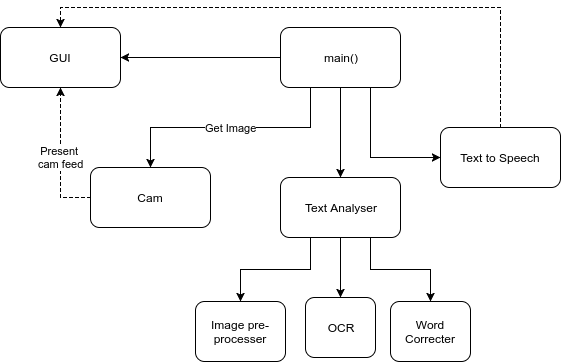
\includegraphics[width=1.0\textwidth]{res/UML1}
\end{figure}

\subsection{GUI}
The graphical interface consists of a windows with various options. It
displays live camera feed and giving options to the user to capture an image
by pressing a button. It has a text field which contains the text after an
image has been analyzed. To be able to implement the camera, OpenCV are used.
The other graphical components are Tkinter objects.

\subsection{Optical character recognition --- OCR}
OCR is the module that turns an image into characters. It is a wrapper for the
Tesseract API, which is a  machine learning-based open source OCR engine that
is maintained by Google. OCR may be implemented from scratch in the future,
using Neural Networks.

\subsection{Text-To-Speech}
TTS is the module that turns text (given from OCR) into speech. The module is
a wrapper for gTTS, which is an interface for Google’s Text-To-Speech API.

\subsection{Tests}
\textit{TBD}

\section{Result}
\textit{TBD}

\section{Discussion}
\textit{TBD}

\pagebreak
% Ask me how to properly insert references // Duane
\bibliography{references}
\bibliographystyle{ieeetr}

\end{document}
